\documentclass[tikz,border=2pt]{standalone}
\usepackage{tikz}
\usepackage{lmodern}
\usetikzlibrary{calc,decorations.pathreplacing}

% Visual conventions follow the existing MRNC TikZ pictures: ordinary
% components use TikZ's normal 0.4pt stroke, with compact TeX labels.
\tikzset{
  nu fibre/.style={
    x=0.78cm,
    y=0.78cm,
    line width=0.4pt,
    line cap=round,
    line join=round
  },
  nu label/.style={
    font=\scriptsize,
    inner sep=1pt
  },
  nu annotation/.style={
    font=\scriptsize,
    inner sep=1pt
  },
  nu dots/.style={
    font=\small,
    inner sep=0pt
  }
}

\begin{document}
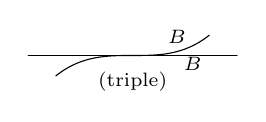
\begin{tikzpicture}[nu fibre]
  \draw (-1.7,0) -- (1.7,0);
  \draw[samples=120,smooth,domain=-1.25:1.25] plot (\x,{0.17*(\x)^3});
  \node[nu label] at (0.72,0.30) {$B$};
  \node[nu label] at (0.98,-0.14) {$B$};
  \node[nu annotation] at (0,-0.42) {$\mathrm{(triple)}$};
\end{tikzpicture}
\end{document}
